\documentclass[runningheads,a4paper]{llncs}

\usepackage{graphicx}
\usepackage{wrapfig}
\usepackage{subfigure}
\usepackage[utf8]{inputenc}
\pagenumbering{roman}
\usepackage{textcomp}
\usepackage{pifont}
\usepackage{color}
\usepackage{blindtext}
\usepackage{enumitem}


\begin{document}
\mainmatter  % start of an individual contribution

%Titel
\title{HCI Meilenstein 4}

\titlerunning{HCI Meilenstein 4}

\author{
  Dursun, Camkerten
  \texttt{a0027244@@unet.univie.ac.at}
  \and
  Pektas, Tarik
  \texttt{a1325165@@unet.univie.ac.at}
  \and
  Bozkurt Yigit Berkay
  \texttt{a1029659@@unet.univie.ac.at}
  \and
  Ayyildiz Mert Ahmet
  \texttt{a1125172@@unet.univie.ac.at}
}

\institute{Universität Wien  / HCI \\
\ SS16 / Gruppe 3 (Freitag) / Team 10}


\maketitle

\section{Usability Test Aufgaben}
Folgende drei Aufgaben wurden für die geplanten Benutzertests ausgewählt.

\begin{itemize}
\item Add new Expense
\item Add new Income
\item Reporting
\end {itemize}


\subsection{Usability Test -1 Add Expense}

Da die Hauptaufgabe unserer App die Verwaltung der Ein und Ausgaben ist, befindet sich die am häufigsten zu benutzende Funktion am der Startseite. Ein Benutzer führt folgende Schritte aus, um eine Ausgabe erfolgreich einzutragen\\\\
•	Paymenttype auswählen:  Aus einem Drop Down Menü wird aus drei Zahlungs-möglichkeiten( Credit Card, Maestro, Cash) die passende ausgewählt.\\\\
•	How much? : Hier wird die Höhe des Betrags in einem Eintagsfeld eingetippt und anschließend bestätigt. Dieses Feld ist erforderlich , um eine Ausgabe erfolgreich abzuschliessen.\\\\
	Die Voraussetzung der Eingabe wird  mit einer Anmerkung (required) signalisiert, bis eine Eingabe stattfindet.\\\\
•	What did you buy?: Ein Textfeld , um eine Eingabe über die Art der Ausgabe einzutippen.\\\\
•	Auswahl des Datums: Hier ist der aktueller Datum bereits ausgewählt. Der Benutzer hat aber auch die Möglichkeit einen anderen Datum auszuwählen.\\\\
•	Clear/Save:Durch ein Klick auf dem Button "Save" werden die Eingabewerte gespeichert. "Clear"-Button löscht die Felder.\\\\



\subsection{Usability Test -2 Add Income}
 Die Funktion Einnahmenverwaltung umfasst die zweitwichtigste Aufgabe unserer Applikation. Um eine neue Einnahme einzufügen, wählt man aus Startseite nach dem Öffnen von dem oben links positionierten Side Panel die erste Funktion "Income". Für einen erfolgreichen neuen Eintrag einer Einnahme sind folgende Schritte in der Applikation vorgesehen.\\

•	Income Type: Auch hier hat man die Möglichkeit durch ein Drop-Down Menü, aus drei Einnahmequellen (salary, debt, other) auszuwählen. \\\\
•	Amount?: In diesem Textfeld wird die Höhe der Einnahme eingetragen, die für einen erfolgreichen Abschluss der Eingabe erforderlich ist.\\\\
•	Auswahl des Datums: ist analog zur Auswahl des Datums bei einer Ausgabe wie oben beschrieben.\\\\
•	Clear/Save: die Aufgabe dieser Buttons ist analog zu den Clear/Save Buttons der Ausgabenfunktion.\\\\




\subsection{Usability Test -3 Reporting}
Aus zu den Berichten gelangt man über SidePanel,  der aus jeder Seite zugreifbar ist. Eine erfolgreiche Berichterstellung durch unsere App sieht folgende Schritte vor:\\\\
•	Bericht auswählen: Hier hat man die Möglichkeit durch Drop Down Menü eine Ausgabenfunktion auszuwählen.\\\\
•	Type: Aus dem Drop Down Feldern kann eine Visualisierungs-werkzeug (Tabelle /Diagramm) ausgewählt werden.\\\\
•	Startdatum/Enddatum eingeben.\\
•	Button "generate report" klicken.\\


\section{Interview Analyse Bericht-Ergebnisse}

Nach Erstellung der vorgesehenen Usability Test Aufgaben für unsere Applikation, wollen wir durch ein Fragenbogenkatalog das Feedback der Testbenutzer  protokollieren.  Wir wollen nach jeder der drei oben beschriebenen Aufgaben  die Erfahrungen der Testbenutzer durch folgende Fragen feststellen.\\

\begin{itemize}
\item Haben Sie die Aufgabe erfolgreich abgeschlossen?\\
\item Haben Sie das Gefühl gehabt, dass bei der Aufgabe eine wichtige Funktion fehlen würde?\\
\item Haben Sie das Gefühl gehabt, dass bei der Aufgabe unnötige Eingaben verlangt wurden?\\
\item Gibt es etwas, was Sie uns mitteilen möchten? (z. Bsp. Verbesserungsvorschläge)\\
\end {itemize}


\subsection{Usability Test: Vorbereitungsphase}


\subsubsection{Zielgruppe}
Unsere Zielgruppe für die Evaluierung unserer Prototypen sind Personen, die der primären Zielgruppe der Anwender unserer Applikation entsprechen. (siehe Personas)

\subsubsection{Wo und Wie}
\begin{itemize}
\item Wir werden unser Prototyp, das auf einem Laptop gespeichert ist, über einen Emulator starten\\
\item Die Aufgaben, die auf einem A4 ausgedruckt sind, werden jeder Testperson erklärt. \\
\item ausgedrucktes Fragenbogen wird zum Ausfüllen bereitgestellt und Testpersonen wird erklärt, wann und welche Fragen beantwortet werden sollen.\\
\end {itemize}
Für die Durchführung der Tests  sind  die Lernräume der Fakultät Informatik vorgesehen.\\

\subsubsection{Testpersonen}
Nachdem wir die Aufgaben definiert haben und auch das Fragebogen zur Evaluierung unserer Applikation erstellt haben, wurden Testpersonen für unsere Finanzapplikation gesucht, die auch zu unserer primären Usergruppe gehörten.\\\\ Hierfür wurden hauptsächlich Studenten der Fakultät Informatik angesprochen.  5 Studierende entschieden sich für die Teilnahme. 
\\
Testdauer:15 min /Testperson vorgesehen.


\subsection{Durchführung der Usability Tests}
Wir haben uns mit allen Testpersonen zu den vereinbarten Zeiten in Lernräumen getroffen. Ihnen wurde der Ablauf der Test noch einmal ausführlich erklärt. Die Testpersonen führten die Aufgaben auf einem Laptop und füllten das Fragebogen aus. \\

Folgende Punkte wurden zusammenfassend aus den ausgefüllten Fragebogen herausgenommen.\\

\begin {itemize}
\item Testpersonen notieren, dass einFeedback nach erfolgreichem Abschluss einer Eintragung in Einnahmen bzw. Ausgaben fehlt.\\
\item Sie finden keine Hilfefunktionen\\
\item Sie konnten kein Geldeinheitszeichen sehen.\\
\item Sie fragen nach Möglichkeit einer Transaktion zwischen App und einer Bank.\\
\item Sie finden Berichte nur für Ausgaben nicht ausreichen und schlagen vor, für Einnahmen auch Berichterstellung.\\
\item Ein Testuser schlug die Möglichkeit der Implementierung einer Sprachsteuerung vor.\\
\end {itemize}



\subsection{Analyse der Usability-Test}

Nach der Durchführung der Usability Tests analysierten wir als Entwicklerteam die Schwachstellen unseres High Fidelity Prototyps und trafen folgende Entscheidungen.\\

\begin {itemize}
\item Einer von 10 Heuristiken von Nielsen ist das Feedback. Daher entschieden wir uns für Implementierung von Feedback nach Abschluss einer Eingabe in Ein und Ausgaben.\\
\item Auch Hilfe und Dokumentation gehört zu den Heuristischen von Nielsen und wir wollen aus diesem Grund Tooltips in die App implementieren.\\
\item Wir erweitern die Funktion Berichterstellung und ermöglichen auch die Berichterstellung von Einnahmen.\\
\item Transaktionen zwischen App und einer Bank erfordert Kenntnisse die über dieses Projekt hinausragen. Außerdem ist die Zusammenarbeit mit Banken erforderlich.\\
\item Auch eine Sprachsteuerung überschreitet den Umfang dieses Projektes.\\
\end {itemize}



\section{Beschreibung des weiterentwickelten Prototypen}
Als erstes wurde die Reporting Seite um die neuen Reports (Income, Targets) erweitert. Damit das richtig funktionieren kann mussten wir einiges anpassen. Im Controller (reportCtrl) gibt es nun für jeden Report eine eigene Funktion die die entsprechenden Spalten hinzufügt. Weiteres wurde der Service, welcher die Abfrage durchführt, um einen Parameter erweitert.\\\\ Somit kann die gleiche Abfrage dynamisch verwendet werden. \\

\begin{figure}
\centering
\subfigure[New Savings Report]{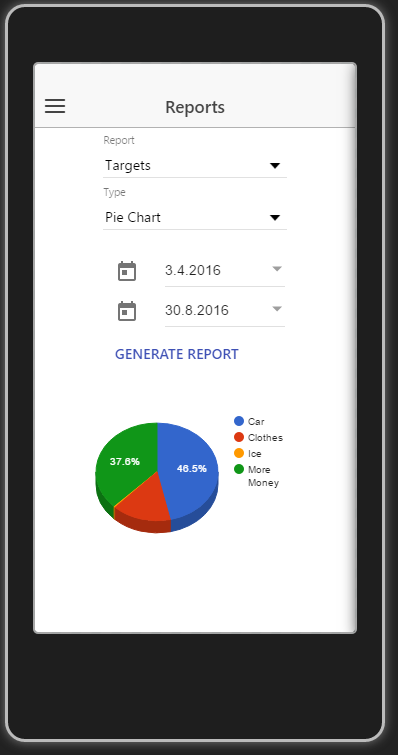
\includegraphics[width=0.15\textwidth]{newSavingTargetReport.png}}
\hfill
\subfigure[New Income Report]{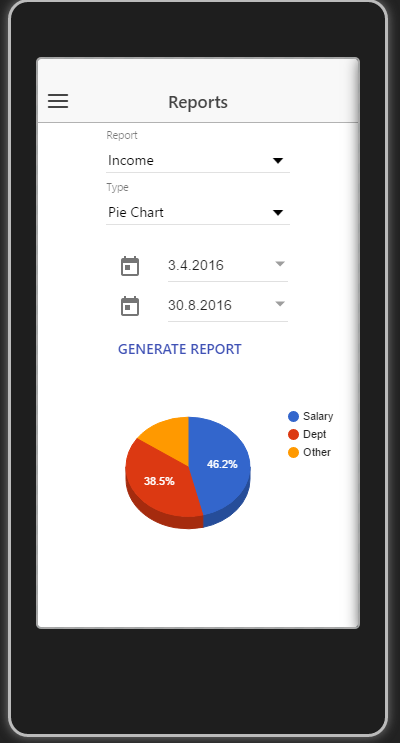
\includegraphics[width=0.15\textwidth]{NewIncomeReport.png}}
\hfill
\subfigure[New Reports]{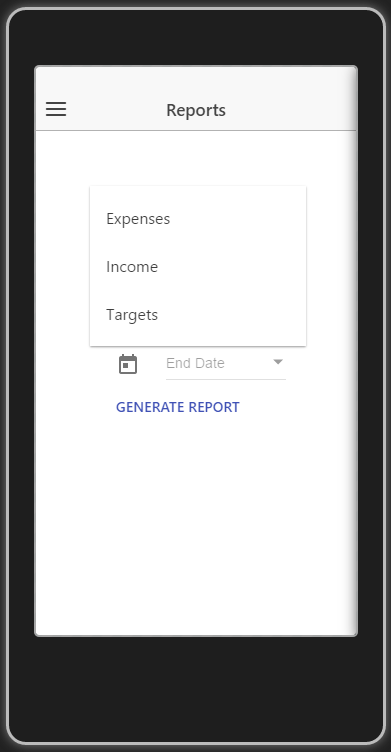
\includegraphics[width=0.15\textwidth]{MultipleReportsMenu.png}}
\end{figure}




Als nächstes haben wir als Ergebnis der Befragung jedes Eingabe Feld nochmals unter die Lupe genommen und für jene, für die es nicht auf dem ersten Blick klar war, kurze Beschreibungen geschrieben. Damit diese Beschreibungen nur bei Bedarf erscheinen haben wir ein kompaktes Icon gesucht und diese als Hover Tooltips eingeblendet.  \\\\ Das Icon sowie die Funktionalitäten haben wir von dem MaterialJS Framework genutzt. Außerdem mussten wir das die entsprechenden CSS Daten einbinden und die Tool Tipps je nach Feld sowie Seite anpassen (wie sie genau eingeblendet werden sollen). \\\\Alle Seiten wurden in diesem Rahmen nochmals überarbeitet (Euro Symbol hinzugefügt, bugs gefixt etc.).

Die letzte größere Implementierung war das Feedback der Formulare welches nach einer erfolgreichen Eingabe nun am Ende der Seite eingeblendet wird. \\\\Wir haben auch ein Event Listener in einen Felder eingestellt welches nach setzen eines Focus die "Success" Nachricht wieder löscht und das Formular in den Ursprungszustand bringt. 



\begin{figure}
\centering
\subfigure[Reporting Tooltip]{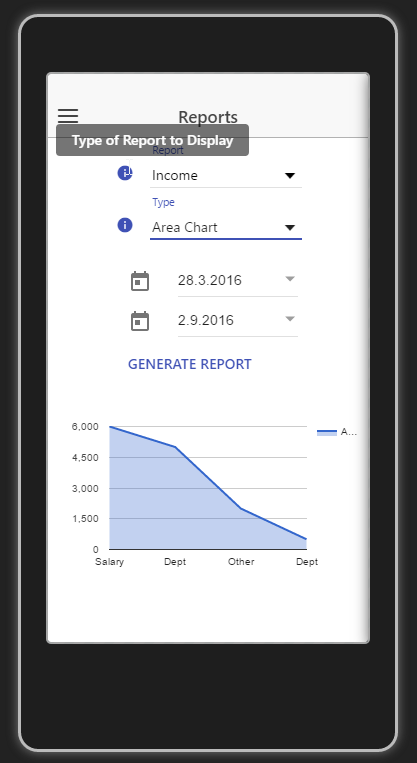
\includegraphics[width=0.13\textwidth]{ReportTooltip.png}}
\hfill
\subfigure[Saving Target Tooltip]{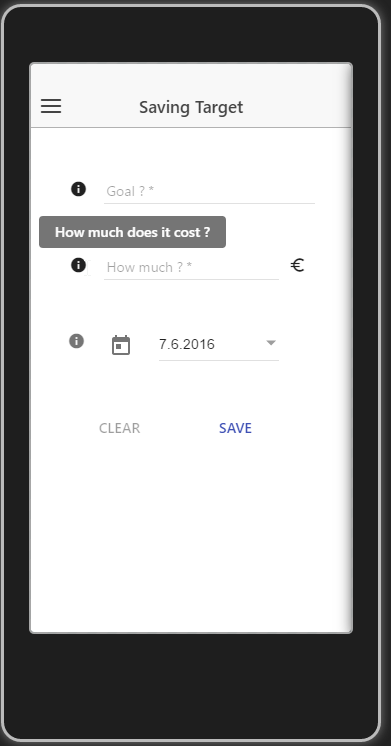
\includegraphics[width=0.13\textwidth]{savingTargetTooltip.png}}
\hfill
\subfigure[ Expense Tooltip]{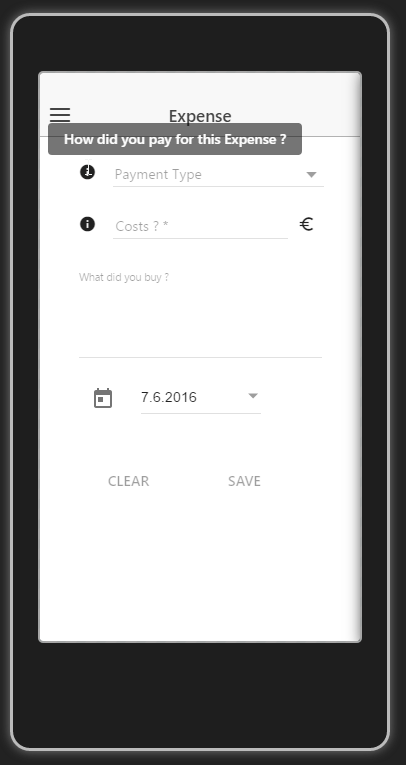
\includegraphics[width=0.13\textwidth]{ExpenseTooltip.png}}
\vfill
\subfigure[Income Tooltip]{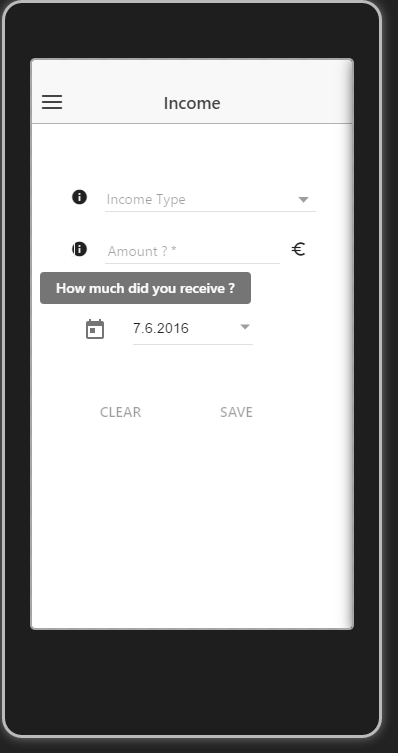
\includegraphics[width=0.13\textwidth]{incomeTooltip.png}}
\hfill
\subfigure[Saving Target Feedback]{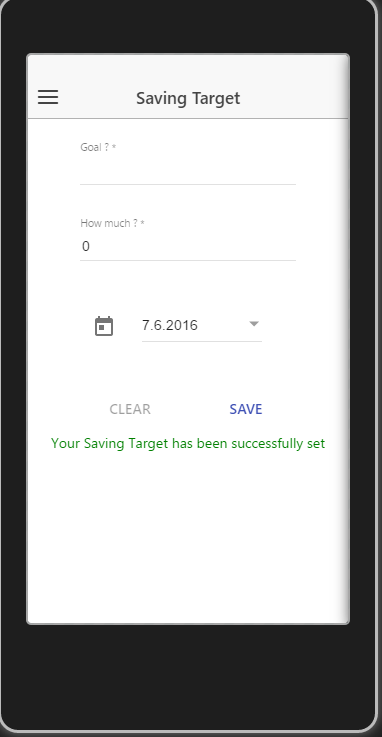
\includegraphics[width=0.13\textwidth]{SavingTargetFeedback.png}}
\hfill
\subfigure[Income added Feedback]{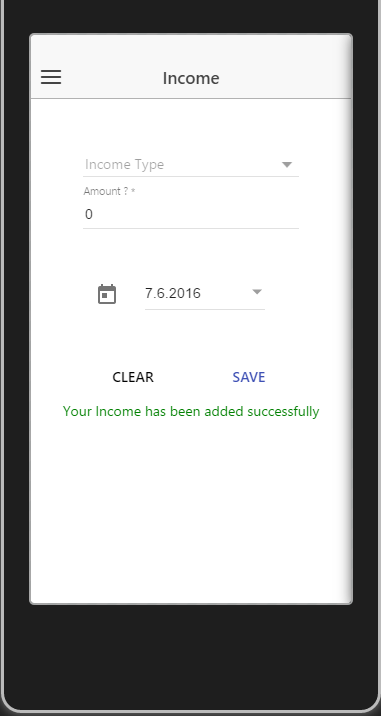
\includegraphics[width=0.13\textwidth]{IncomeAddedFeedback.png}}
\hfill
\subfigure[Expense added Feedback]{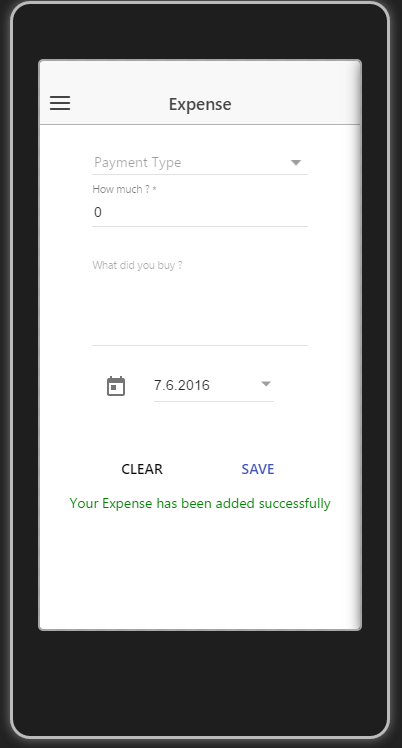
\includegraphics[width=0.13\textwidth]{ExpenseAddedFeedback.png}}
\end{figure}



\section{Arbeitsverteilung- Interne Abläufe}
Wir haben uns generell jede Arbeit so aufgeteilt, so dass jedem, ungefähr gleich viel Last entstanden ist. Natürlich, hat sich das auch so entwickelt, dass sich jeder in seiner Stärken mehr eingesetzt hat. Daher kam es natürlich dazu, dass einer vielleicht mehr programmierte und die anderen sich mehr auf Schreibarbeiten konzentrierten. \\\\Jedenfalls waren wir ein Team das sich eigentlich ziemlich gut verstanden hat. Kommunikation lief hauptsächlich über Facebook. Wir hatten eine gruppe für HCI erstellt. Außerdem haben wir uns jeden Freitag nach der Lehrveranstaltung zusammengesetzt. \\\\Für Code und Dokumente haben wir in Git ein Repository erstellt und dies genutzt.  Die Arbeitslast war Zeit zu Zeit doch etwas hoch aber der Lernprozess lief auch entsprechend parallel hierzu. Alles in allem haben wir uns sicherlich weiterentwickeln können und sind auch somit zufrieden. 


\end{document}